% ============================================================================================================
% C4AI4C'27 (ICASSP 2027 Satellite Workshop) -- AUTHOR-READY SKELETON, NOT A MANUSCRIPT.
% Built on the official ICASSP 2027 template (template_official/Template.tex; spconf.sty, IEEEbib.bst copied
% unmodified from ICASSP2027_Paper_Templates.zip, SHA-256 fd1cc410...).
% Contains: section headings, page budget, author notes, verified equations, generated tables/figures,
% captions marked AUTHOR REVIEW REQUIRED, verified references. All scientific prose must be written by the
% authors. Every result sentence must map to paper_plan/32_final_claim_matrix.md and CLAIM_EVIDENCE_CHECKLIST.md.
% Limits (verified, doc 36): 4 pages of content + 1 page (references, funding acknowledgements, Compliance with
% Ethical Standards only); single-blind (author names in the PDF); abstract ~100-150 words; <= 5 keywords;
% every author needs an ORCID iD; AI-generated content disclosed in the acknowledgments.
% ============================================================================================================
\documentclass{article}
\usepackage{spconf,amsmath,amssymb,graphicx,hyperref,xcolor}

% ---- author notes: visible in drafts; set \shownotesfalse (or delete every \authornote) before submission ----
\newif\ifshownotes \shownotestrue
\newcommand{\authornote}[1]{\ifshownotes{\color{blue}\footnotesize[AUTHOR NOTE: #1]}\fi}

\title{Detection Is Not Attribution: Reference Contamination and False Client Accusations in Federated Learning Forensics}
% AUTHOR: confirm the final title (approved working title, P-59/P-61).

\name{AUTHOR NAMES (every author must have an ORCID iD)}
\address{AUTHOR AFFILIATIONS}

\begin{document}
\ninept
\maketitle

\begin{abstract}
\authornote{Write 100--150 words; must be identical to the portal abstract (portal limit 200 words). Required
content, in this order: (1) the question -- when do FL anomaly detectors fail to identify the right client or to
separate poisoning from benign drift; (2) the setting -- few-client cross-silo FedAvg, CIFAR-100, matched clean /
BadNets / benign-drift interventions, four seeds of which two preregistered; (3) the main findings, each worded as in
paper\_plan/32 (C-01 ... C-07); (4) the conditional mechanism, stated as observed in one development seed; (5) no
claim of a new detector.}
\end{abstract}

\begin{keywords}
% AUTHOR: <= 5 keywords, identical to the portal entry. Suggestions to review: federated learning, data poisoning,
% forensic attribution, benign distribution drift, change detection.
KEYWORD1, KEYWORD2, KEYWORD3, KEYWORD4, KEYWORD5
\end{keywords}

% ------------------------------------------------------------------------------------------------ 0.55 page
\section{Introduction}
\label{sec:intro}
\authornote{Budget 0.55 page. Motivate client-level forensics in few-client (cross-silo) FL with plaintext updates;
define the five outcomes kept separate throughout: attack effectiveness, detection, source attribution,
onset localisation, honest-client false accusation. State the research question (doc 35 \S1). List at most three
contributions exactly as approved in paper\_plan/33 \S1 (C1 reliability decomposition and matched evaluation;
C2 cross-seed outcomes; C3 conditional reference-contamination analysis). Do not call FedTrace v3 a proposed or
superior detector (P-63): it is the evaluated framework.}

% ------------------------------------------------------------------------------------------------ 0.35 page
\section{Relation to Prior Work}
\label{sec:prior}
\authornote{Mandatory per the official template. Budget 0.35 page. Use only the verified statements in
paper\_plan/36 \S6 and doc 20: FLTracer~\cite{zhang2024fltracer} already performs online per-client attribution
with an attack time and type, and states that abruptly shifting benign clients are sacrificed; FLDetector~\cite{zhang2022fldetector}
scores per-client update consistency (no onset); DeepSight~\cite{rieger2022deepsight} addresses static benign
non-IID data for backdoors; FLForensics~\cite{jia2025flforensics} traces clients post hoc; FedREDefense~\cite{xie2024fedredefense}
excludes data poisoning; CUSUM~\cite{page1954cusum} and related change detection are standard. Say what is NOT new
(median algebra, z-scores, CUSUM). No numerical comparison with methods we did not run.}

% ------------------------------------------------------------------------------------------------ 0.6 page
\section{Problem Setting and Evaluated Framework}
\label{sec:method}
\authornote{Budget 0.6 page. Observation model (doc 15 A1): the server sees every client's submitted state and the
pre-round global model; nothing about data or labels. Define the outcomes. Then FedTrace v3 in the equations below
(verified against src/analysis/fedtrace\_detector.py, frozen at 7f6ca8b), followed by the baselines (ZP-norm,
CUSUM-norm; thresholds from the development clean runs, L-56).}

% ---- VERIFIED EQUATIONS (frozen v3; doc 25 \S1). AUTHOR: keep notation consistent with the text. ----
For client $k$ in round $r$, let $n_k(r)$ be the update norm and $t_k(r)$ the cosine between the client's updates in
rounds $r$ and $r-1$. With the client's own sample mean and standard deviation over rounds $0\le r<T_{\mathrm{ref}}=20$
for the norm and $1\le r<T_{\mathrm{ref}}$ for the residual,
\begin{align}
z^m_k(r) &= \frac{|n_k(r)-\mu^m_k|}{\sigma^m_k}, \qquad
c(r) = \operatorname{med}\{t_1(r),\dots,t_K(r)\}, \qquad d_k(r) = c(r) - t_k(r), \label{eq:scores}\\
z^t_k(r) &= \max\!\Big(0,\; \frac{d_k(r)-\mu^d_k}{\sigma^d_k}\Big), \qquad
S_k(r) = \max\big(z^m_k(r),\, z^t_k(r)\big). \label{eq:score}
\end{align}
A client is confirmed at round $a$ if $S_k(r)\ge\tau=3$ for $P=3$ consecutive rounds ending at $a$; the attributed
client is the first confirmed one and the onset estimate is the first round of its confirming streak.
\authornote{Verified against compute\_all\_scores\_v3 (z\_m = abs(n - mean)/std; residual one-sided; sample
standard deviations; calibration windows as stated).}

% ------------------------------------------------------------------------------------------------ 0.45 page
\section{Reference Contamination}
\label{sec:contamination}
\authornote{Budget 0.45 page. State clearly that Eq.~(\ref{eq:clip}) is an elementary property of the median, not
a contribution; the contribution is the forensic consequence and its cross-seed check (doc 25, doc 29).}
Fix the other $K-1$ values sorted as $s_1\le\dots\le s_{K-1}$. For odd $K=2m-1$ the inclusive median, as a function
of client $j$'s value $x$, is
\begin{equation}
c(x) = \min\!\big(\max(x,\, s_{m-1}),\, s_m\big), \label{eq:clip}
\end{equation}
so $j$ moves the reference only if it enters, leaves or crosses the band $[s_{m-1},s_m]$. Every other client's
residual then shifts by the same $\Delta c_j$, i.e.\ by $\Delta c_j/\sigma^d_k$ in the units of Eq.~(\ref{eq:score});
because $z^t$ is one-sided, only an upward crossing can raise an honest client's score, and the displacement is
necessary for an honest confirmation at round $a$ iff
\begin{equation}
\exists\, r\in\{a-P+1,\dots,a\}:\;\max\!\Big(z^m_k(r),\; \max\big(0,\, z_k(r)-\Delta c_j(r)/\sigma^d_k\big)\Big) < \tau,
\label{eq:necessity}
\end{equation}
where $z_k$ is the signed residual score before truncation. \authornote{Report: observed in development seed 2026
only, where client\_002 was the pre-onset median client (rank 3 of 5); in 123, W1, W2 it started above the band
(rank 4) and no contamination occurred (C-05, C-06). The deployable proxy did not generalise (C-08).}

% ------------------------------------------------------------------------------------------------ 0.35 page
\section{Experimental Protocol}
\label{sec:setup}
\authornote{Budget 0.35 page. CIFAR-100, ResNet-18 (CIFAR variant), $K=5$, full participation, 50 rounds, one local
epoch, Dirichlet $\alpha=0.1$; intervened client client\_002 from round 20; BadNets (target class 0, 50\% of its
non-target samples, $3\times3$ patch); benign class-composition drift (protocol 13); matched arms with
bit-identical pre-intervention histories; seeds 123 and 2026 (development) and W1, W2 (preregistered,
protocol 26); thresholds frozen; FedAvg~\cite{mcmahan2017fedavg}; BadNets~\cite{gu2019badnets}. Model and dataset
citations are placeholders in refs.bib (unverified).}

% ------------------------------------------------------------------------------------------------ 1.2 pages
\section{Results}
\label{sec:results}
\authornote{Budget 1.2 pages incl.\ Table~\ref{tab:seedlevel} and Figs.~\ref{fig:contamination}--\ref{fig:grid}.
Write one paragraph per outcome, each sentence mapped to a claim ID in paper\_plan/32: attack effectiveness (C-07),
detection and attribution (C-01, C-02), benign drift (C-03), threshold transfer (C-04), contamination (C-05,
C-06), proxy (C-08). Archived perturbation results only as one sentence of context (C-11), labelled as model-update
perturbations, not poisoning.}

% GENERATED by manuscript_c4ai4c27/scripts/make_assets.py from frozen artifacts -- do not edit by hand.
\begin{table*}[t]
\centering\footnotesize
\setlength{\tabcolsep}{3pt}
\begin{tabular}{llrrlllll}
\hline
Arm & Seed & ASR & $\Delta$top-1 & v3 & v3 magnitude-only & v3 t\_res-only & ZP-norm & CUSUM-norm \\
\hline
BadNets & 123 & 43.5\% & -1.94 & \checkmark\ 8/10 & \checkmark\ 8/10 & missed & \checkmark\ 1/3 & \checkmark\ 0/6 \\
BadNets & 2026 & 64.7\% & -0.94 & $\times$ first 4; FA\,1,4 & \checkmark\ 2/4 & missed; FA\,1,4 & \checkmark\ 0/2 & \checkmark\ 0/5 \\
BadNets & W1$^\ast$ & 63.3\% & -0.96 & missed & missed & missed & \checkmark\ 1/3; FA\,4 & \checkmark\ 0/6; FA\,4 \\
BadNets & W2$^\ast$ & 44.2\% & -0.86 & missed & missed & missed & \checkmark\ 1/3 & \checkmark\ 0/6 \\
\hline
drift & 123 & 0.6\% & -1.75 & -- & -- & -- & \textbf{acc.\,}2 & \textbf{acc.\,}2 \\
drift & 2026 & 0.2\% & -1.79 & \textbf{acc.\,}1,4 & -- & \textbf{acc.\,}1,4 & \textbf{acc.\,}1 & \textbf{acc.\,}2 \\
drift & W1$^\ast$ & 0.7\% & -2.29 & \textbf{acc.\,}2 & \textbf{acc.\,}2 & -- & \textbf{acc.\,}2,4 & \textbf{acc.\,}2,4 \\
drift & W2$^\ast$ & 0.1\% & -1.47 & -- & -- & -- & \textbf{acc.\,}2 & \textbf{acc.\,}2 \\
\hline
clean & 123 & 0.7\% &  & -- & -- & -- & -- & -- \\
clean & 2026 & 0.3\% &  & -- & -- & -- & -- & -- \\
clean & W1$^\ast$ & 0.8\% &  & -- & -- & -- & \textbf{acc.\,}4 & \textbf{acc.\,}4 \\
clean & W2$^\ast$ & 0.0\% &  & -- & -- & -- & -- & -- \\
\hline
\end{tabular}
\caption{AUTHOR REVIEW REQUIRED. Seed-level outcomes (no pooling). $^\ast$ preregistered confirmation seeds (W1 = 1178015705, W2 = 1463065807); 123, 2026 development seeds. Malicious arm cells: \checkmark\ = attacker confirmed first, onset error / delay in rounds; $\times$ = an honest client confirmed first; FA = honest clients confirmed (index). Drift / clean cells: acc. = clients confirmed (all honest; in drift client 2 is the intervened honest client). ASR = triggered attack success on 9,900 non-target test images; criterion $\geq$ 50\%. Thresholds frozen (v3 $\tau=3$, $P=3$; ZP $h=1.75$, CUSUM $h=11.75$ from development clean runs).}
\label{tab:seedlevel}
\end{table*}


\begin{figure*}[t]
\centering
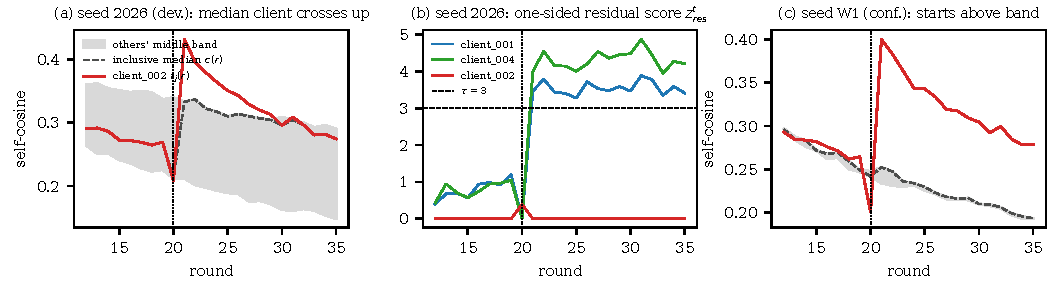
\includegraphics[width=\textwidth]{figures/fig1_reference_contamination.pdf}
\caption{AUTHOR REVIEW REQUIRED. (a) Development seed 2026, BadNets: client\_002 (red) is the pre-onset median
client; after onset its self-cosine rises above the other clients' middle band (grey) and the inclusive median
(dashed) moves up. (b) The one-sided residual scores of honest client\_001 and client\_004 exceed $\tau=3$ from
round 21 and they are confirmed at round 23, before the attacker. (c) Confirmation seed W1: client\_002 starts above
the band, so its rise leaves the median unchanged. Generated from frozen traces (ASSET\_PROVENANCE.json).}
\label{fig:contamination}
\end{figure*}

\begin{figure*}[t]
\centering
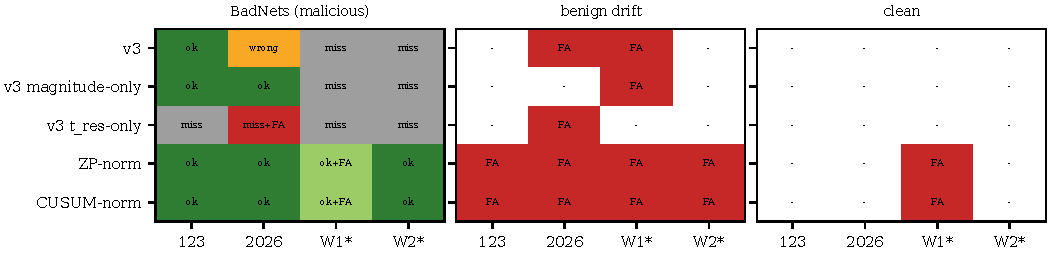
\includegraphics[width=\textwidth]{figures/fig2_reliability_grid.pdf}
\caption{AUTHOR REVIEW REQUIRED. Outcome per seed and detector (no pooling). ok: attacker confirmed first, no honest
alarm; ok+FA: attacker first but an honest client also confirmed; wrong: an honest client confirmed first; miss:
attacker never confirmed; FA: honest client(s) confirmed. $^\ast$ preregistered confirmation seeds. Frozen
thresholds; generated from frozen outcome tables (ASSET\_PROVENANCE.json).}
\label{fig:grid}
\end{figure*}

% ------------------------------------------------------------------------------------------------ 0.3 page
\section{Limitations and Conclusion}
\label{sec:conclusion}
\authornote{Budget 0.3 page. Must state (doc 34): four seeds (two preregistered) -- no rates; one dataset, model,
$K$, intervened client, onset (= $T_{\mathrm{ref}}$), drift type; two of four BadNets runs below the 50\% ASR
criterion; norm thresholds calibrated on clean runs of the development seeds; the contamination mechanism observed
once; malicious intent not identifiable from updates without assumptions on benign data (doc 15 A3--A4); no
FLTracer / FLDetector execution.}

% ---- page 5: references, funding acknowledgements and Compliance with Ethical Standards ONLY ----
\section{Compliance with Ethical Standards}
\authornote{AUTHOR: write the statement (e.g.\ public dataset, no human subjects) -- verify requirement wording.}

\section{Acknowledgments}
\authornote{AUTHOR: funding. AI-use disclosure is REQUIRED by the ICASSP 2027 / IEEE policy for AI-generated
content (text, figures, images, code): name the AI system (Claude, Anthropic) and the specific parts it produced or
assisted (see paper\_plan/36 \S4 inventory), and the level of use. Note: under the ICASSP 5th-page rule the
acknowledgments content on page 5 should be funding; confirm with the organisers where the AI disclosure must sit if
it would push content beyond 4 pages.}

\bibliographystyle{IEEEbib}
\bibliography{refs}

\end{document}
